\chapter{Droites du plan}

\section{Qu'est-ce qu'une équation de droite ?}

\begin{definition}[Équation d'une droite]
	Dans le plan muni d'un repère $\vOIJ$, une \textbf{équation d'une droite} $d$ est une relation algébrique reliant les coordonnées $\coordl{x}{y}$ des points du plan.

	Un point $M\coordl{x}{y}$ appartient à la droite $d$ \textbf{si et seulement si} ses coordonnées vérifient cette relation. On note alors :
	\[
		M\coordl{x}{y} \in d \iff \text{les coordonnées }\coordl{x}{y}\text{ vérifient l'équation de }d
	\]
\end{definition}

\begin{ex}
	Soit $d$ la droite d'équation $2x - 3y + 1 = 0$.
	\begin{itemize}
		\item Le point $A\coordl{1}{1}$ appartient-il à $d$ ?
		      \[
			      2 \times 1 - 3 \times 1 + 1 = 2 - 3 + 1 = 0
		      \]

		      Les coordonnées de $A$ vérifient l'équation, donc $A(1\,;\,1) \in d$.

		\item Le point $B\coordl{2}{1}$ appartient-il à $d$ ?
		      \[
			      2 \times 2 - 3 \times 1 + 1 = 4 - 3 + 1 = 2 \neq 0
		      \]

		      Les coordonnées de $B$ ne vérifient pas l'équation, donc $B(2\,;\,1) \notin d$.
	\end{itemize}
\end{ex}

\begin{remarque}
	Une même droite $d$ peut s'exprimer sous plusieurs formes d'équations :

	\begin{itemize}
		\item La \textbf{forme réduite} : $y = mx + p$ (ou $x = k$), vue en $3^\text{e}$.
		\item La \textbf{forme cartésienne} : $ax + by + c = 0$, que nous allons étudier dans ce chapitre.
	\end{itemize}
\end{remarque}

\section{Équation réduite et pente d'une droite}

\subsection{Équation réduite d'une droite}

\begin{prop}[Équation réduite]
	\nline
	\begin{wrapstuff}[r]
		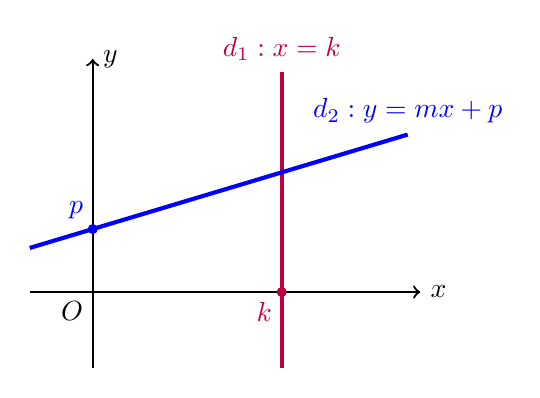
\begin{tikzpicture}[scale=0.8]
			\draw[thick,->] (-1,0) -- (5.2,0) node[right] {$x$};
			\draw[thick,->] (0,-1.2) -- (0,3.7) node[right] {$y$};
			\node[below left] at (0,0) {$O$};
			\draw[line width=1.5pt, purple] (3,-1.2) -- (3,3.5) node[above] {$d_1 : x = k$};
			\filldraw[purple] (3,0) circle (2pt) node[below left] {$k$};
			\draw[line width=1.5pt, blue, domain=-1:5] plot (\x, {0.3*\x + 1}) node[above, sloped] {$d_2 : y = mx + p$};
			\filldraw[blue] (0,1) circle (2pt) node[above left] {$p$};
		\end{tikzpicture}
	\end{wrapstuff}

	Toute droite $d$ du plan admet une unique équation, appelée \textbf{équation réduite}, de l'une des deux formes suivantes :

	\begin{itemize}
		\item Si $d$ est parallèle à l'axe des ordonnées, son équation réduite est de la forme :
		      \[
			      x = k \quad (k \in \R)
		      \]
		\item Si $d$ n'est pas parallèle à l'axe des ordonnées, son équation réduite est de la forme :
		      \[
			      y = mx + p \quad (m, p \in \R)
		      \]
	\end{itemize}
\end{prop}

\begin{definition}[Vocabulaire]
	Pour une droite $d$ d'équation réduite $y = mx + p$ :
	\begin{itemize}
		\item Le réel $m$ est appelé la \textbf{pente} ou le \textbf{coefficient directeur} de la droite $d$.
		\item Le réel $p$ est appelé l'\textbf{ordonnée à l'origine} de la droite $d$.
	\end{itemize}
\end{definition}

\subsection{Calcul du coefficient directeur}

\begin{prop}[Calcul de la pente par deux points]
	Soient $A\coordl{x_A}{y_A}$ et $B\coordl{x_B}{y_B}$ deux points distincts d'une droite $d$.

	Si $x_A \neq x_B$, la droite $d$ n'est pas parallèle à l'axe des ordonnées et son coefficient directeur $m$ est :
	\[
		m = \frac{y_B - y_A}{x_B - x_A}
	\]

	\begin{center}
		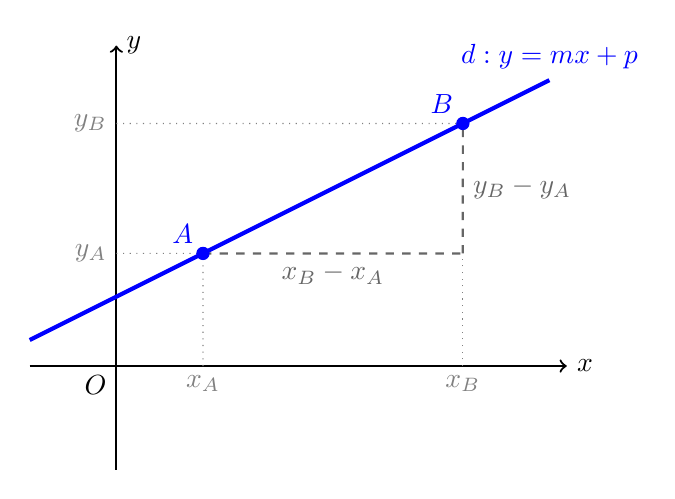
\begin{tikzpicture}[scale=1.1]
			\draw[thick,->] (-1,0) -- (5.2,0) node[right] {$x$};
			\draw[thick,->] (0,-1.2) -- (0,3.7) node[right] {$y$};
			\node[below left] at (0,0) {$O$};
			\coordinate (A) at (1,1.3);
			\coordinate (B) at (4,2.8);
			\draw[line width=1.5pt, blue, domain=-1:5] plot (\x, {0.5*\x + 0.8}) node[above, sloped] {$d : y = mx + p$};
			\draw[dashed, thick, black!60] (A) -- (4,1.3) node[midway, below] {$x_B - x_A$};
			\draw[dashed, thick, black!60] (4,1.3) -- (B) node[midway, right] {$y_B - y_A$};
			\draw[dotted, gray] (1,0) node[below] {$x_A$} -- (A);
			\draw[dotted, gray] (4,0) node[below] {$x_B$} -- (4,1.3);
			\draw[dotted, gray] (0,1.3) node[left] {$y_A$} -- (A);
			\draw[dotted, gray] (0,2.8) node[left] {$y_B$} -- (B);
			\filldraw[blue] (A) circle (2pt) node[above left] {$A$};
			\filldraw[blue] (B) circle (2pt) node[above left] {$B$};
		\end{tikzpicture}
	\end{center}
\end{prop}

\begin{meth}[Établir l'équation réduite à partir de deux points]
	\nline
	\begin{wrapstuff}[r]
		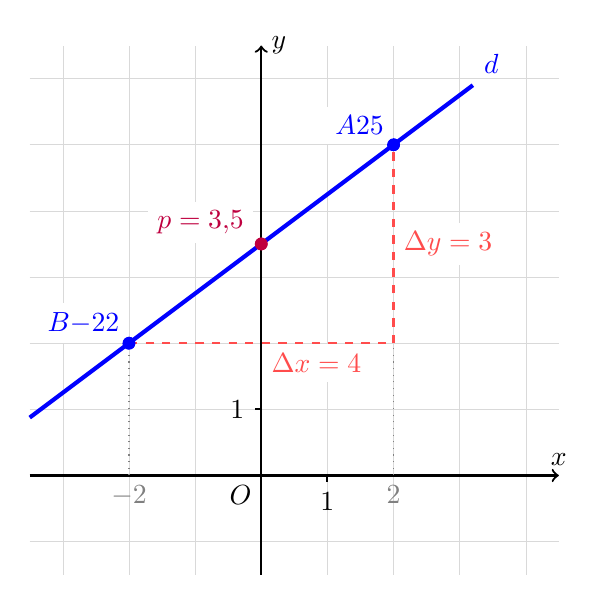
\begin{tikzpicture}[scale=0.84]
			\draw[step=1cm,gray!30,very thin] (-3.5,-1.5) grid (4.5,6.5);
			\draw[thick,->] (-3.5,0) -- (4.5,0) node[above] {$x$};
			\draw[thick,->] (0,-1.5) -- (0,6.5) node[right] {$y$};
			\node[below left] at (0,0) {$O$};
			\draw[thick] (1,0) -- (1,-0.1) node[below] {$1$};
			\draw[thick] (0,1) -- (-0.1,1) node[left] {$1$};
			\draw[line width=1.5pt, blue, domain=-3.5:3.2] plot (\x, {0.75*\x + 3.5}) node[above right] {$d$};
			\draw[dashed, thick, red!70] (-2,2) -- (2,2) node[midway, below, xshift=7mm, fill=white] {$\Delta x = 4$};
			\draw[dashed, thick, red!70] (2,2) -- (2,5) node[midway, right, fill=white] {$\Delta y = 3$};
			\draw[dotted, gray] (-2,0) node[below] {$-2$} -- (-2,2);
			\draw[dotted, gray] (2,0) node[below] {$2$} -- (2,2);
			\filldraw[blue] (-2,2) circle (2.5pt) node[above left, fill=white] {$B\coordl{-2}{2}$};
			\filldraw[blue] (2,5) circle (2.5pt) node[above left, fill=white] {$A\coordl{2}{5}$};
			\filldraw[purple] (0,3.5) circle (2.5pt) node[above left,xshift=-1mm, fill=white] {$p = 3{,}5$};
			\filldraw[blue] (-2,2) circle (2.5pt);
			\filldraw[blue] (2,5) circle (2.5pt);
			\filldraw[purple] (0,3.5) circle (2.5pt);
		\end{tikzpicture}
	\end{wrapstuff}

	Déterminer l'équation réduite de la droite $d$ passant par les points $A\coordl{2}{5}$ et $B\coordl{-2}{2}$.

	\begin{correction}
		Comme $x_A = 2$ et $x_B = -2$, on a $x_A \neq x_B$ donc $d$ admet une équation de la forme $y = mx + p$.

		\begin{enumerate}
			\item \textbf{Calcul du coefficient directeur $m$ :}
			      \[
				      m = \frac{y_A - y_B}{x_A - x_B} = \frac{5 - 2}{2 - (-2)} = \frac{3}{4}
			      \]

			      L'équation s'écrit donc $y = \dfrac{3}{4}x + p$.
		\end{enumerate}

		\begin{enumerate}[resume]
			\item \textbf{Calcul de l'ordonnée à l'origine $p$ :}

			      Le point $A\coordl{2}{5}$ appartient à $d$, ses coordonnées vérifient son équation :
			      \begin{align*}
				      y_A = \frac{3}{4}x_A + p & \eqv 5 = \frac{3}{4} \times 2 + p                                              \\
				                               & \eqv 5 = \frac{3}{2} + p \qquad \eqv p = 5 - \frac{3}{2} = \frac{7}{2} = 3{,}5
			      \end{align*}
		\end{enumerate}

		L'équation réduite de $d$ est $y = \dfrac{3}{4}x + \dfrac{7}{2}$ (ou $y = 0{,}75x + 3{,}5$).
	\end{correction}
\end{meth}

\subsection{Parallélisme avec les équations réduites}

\begin{prop}[Critère de parallélisme]
	Soient deux droites $d$ et $d'$ d'équations réduites respectives $y = mx + p$ et $y = m'x + p'$.
	\begin{itemize}
		\item $d$ et $d'$ sont parallèles si et seulement si elles ont le même coefficient directeur :
		      \[
			      d \parallel d' \eqv m = m'
		      \]
		\item $d$ et $d'$ sont sécantes si et seulement si leurs coefficients directeurs sont différents ($m \neq m'$).
	\end{itemize}
\end{prop}

\begin{methode}[Déterminer la position relative de deux droites]
	Pour déterminer si deux droites non verticales sont parallèles ou sécantes :
	\begin{enumerate}
		\item On identifie ou on calcule leur coefficient directeur (pente).
		\item Si les coefficients directeurs sont égaux, les droites sont \textbf{parallèles}.
		\item S'ils sont différents, les droites sont \textbf{sécantes}.
	\end{enumerate}
\end{methode}

\begin{exemple}
	On considère les trois droites suivantes :
	\begin{multicols}{3}
		\begin{itemize}
			\item $d_1 : y = 2x - 1$
			\item $d_2 : y = 2x + 3$
			\item $d_3 : y = -x + 2$
		\end{itemize}
	\end{multicols}
	\begin{enumerate}
		\item \textbf{Position relative de $d_1$ et $d_2$ :}

		      Le coefficient directeur de $d_1$ est $m_1 = 2$ et celui de $d_2$ est $m_2 = 2$.

		      Comme $m_1 = m_2$, les droites $d_1$ et $d_2$ sont donc \textbf{parallèles} ($d_1 \parallel d_2$).

		\item \textbf{Position relative de $d_1$ et $d_3$ :}

		      Le coefficient directeur de $d_3$ est $m_3 = -1$.

		      Comme $m_1 \neq m_3$ ($2 \neq -1$), les droites $d_1$ et $d_3$ sont donc \textbf{sécantes}.
	\end{enumerate}

	\begin{center}
		\begin{tikzpicture}[scale=0.75]
			% Grille et repère
			\draw[step=1cm,gray!30,very thin] (-3.5,-2.5) grid (4.5,5.5);
			\draw[thick,->] (-3.2,0) -- (4.3,0) node[right] {$x$};
			\draw[thick,->] (0,-2.2) -- (0,5.3) node[above] {$y$};
			\node[below left] at (0,0) {$O$};
			\draw[thick] (1,0) -- (1,-0.1) node[below] {$1$};
			\draw[thick] (0,1) -- (-0.1,1) node[left] {$1$};
			\draw[line width=1.5pt, blue, domain=-0.7:2.8] plot (\x, {2*\x - 1}) node[above right] {$d_1$};
			\draw[line width=1.5pt, red, domain=-2.7:0.8] plot (\x, {2*\x + 3}) node[above right] {$d_2$};
			\draw[line width=1.5pt, codegreen, domain=-3.2:3.8] plot (\x, {-\x + 2}) node[right] {$d_3$};
			\filldraw[blue] (0,-1) circle (2pt) node[right] {$-1$};
			\filldraw[red] (0,3) circle (2pt) node[left] {$3$};
			\filldraw[codegreen] (0,2) circle (2pt) node[above right] {$2$};
		\end{tikzpicture}
	\end{center}
\end{exemple}

\section{Vecteurs directeurs et équations cartésiennes}

\subsection{Vecteur directeur d'une droite}

\begin{df}[Vecteur directeur]
	Soit $d$ une droite du plan.

	On appelle \textbf{vecteur directeur} de $d$ tout vecteur non nul $\vec{u}$ qui possède la même direction que la droite $d$.
\end{df}

\begin{center}
	\begin{tikzpicture}[scale=0.5]
		\draw[line width=1.2pt, domain=-2:4] plot (\x, {0.6*\x + 1}) node[right] {$d$};
		\draw[line width=1.5pt, -Stealth] (-0.5, 2.2) -- (2.5, 4) node[midway, above left] {$\vec{u}$};
	\end{tikzpicture}
\end{center}

\begin{remarque}
	\nline
	\begin{itemize}
		\item Un vecteur directeur n'est jamais nul par définition.
		\item Une droite admet une infinité de vecteurs directeurs. Si $\vec{u}$ est un vecteur directeur de $d$, alors pour tout réel non nul $k$, le vecteur $k\vec{u}$ est aussi un vecteur directeur de $d$.
		\item Pour deux points distincts $A$ et $B$ d'une droite $d$, le vecteur $\vec{AB}$ constitue un vecteur directeur de $d$.
	\end{itemize}
\end{remarque}

\begin{methode}[Déterminer graphiquement un vecteur directeur]
	Pour lire graphiquement un vecteur directeur d'une droite $d$ :
	\begin{enumerate}
		\item Repérer deux points $A$ et $B$ de la droite placés sur des intersections du quadrillage.
		\item Déterminer le déplacement horizontal $\Delta x$ et le déplacement vertical $\Delta y$ pour aller de $A$ à $B$.
		\item Le vecteur $\vec{u}\coord{\Delta x}{\Delta y}$ est un vecteur directeur de $d$.
	\end{enumerate}
\end{methode}

\begin{exemple}
	Dans le repère $\vOIJ$ ci-dessous, la droite $d$ passe par les points $A\coordl{-1}{1}$ et $B\coordl{2}{3}$.

	\begin{center}
		\begin{tikzpicture}[scale=0.9]
			\draw[dotted, gray!40!black] (-3,-1) grid (4,4);
			\draw[gray!20!black,->, thick] (-3,0) -- (4,0) node[above] {$x$};
			\draw[gray!20!black,->, thick] (0,-1) -- (0,4) node[right] {$y$};
			\node[below left] at (0,0) {$O$};
			\draw[thick, ->] (0,0) -- (1,0) node[midway, below] {$\vec{i}$};
			\draw[thick, ->] (0,0) -- (0,1) node[midway, left] {$\vec{j}$};
			\draw[line width=1pt, codeblue, domain=-3:3.5] plot (\x, {2/3*\x + 5/3});
			\node[codeblue, above left] at (-2,0.3) {$d$};
			\draw[ultra thick, ->, green!50!black] (-1,1) -- (2,3) node[midway, above, sloped] {$\vec{u}$};
			\draw[dashed, gray, thick] (-1,1) -- (2,1) node[midway, below] {$+3$};
			\draw[dashed, gray, thick] (2,1) -- (2,3) node[midway, right] {$+2$};
			\filldraw[red] (-1,1) circle (2pt) node[above left] {$A$};
			\filldraw[red] (2,3) circle (2pt) node[above left] {$B$};
		\end{tikzpicture}
	\end{center}

	Le vecteur $\vec{u} = \vec{AB}\coord{3}{2}$ est un vecteur directeur de la droite $d$.
\end{exemple}

\subsection{Équation cartésienne d'une droite}

\begin{prop}[Existence d'une équation cartésienne]
	Dans le plan muni d'un repère $\vOIJ$, toute droite $d$ admet une équation de la forme :
	\[
		ax + by + c = 0
	\]

	où $a$, $b$ et $c$ sont des réels tels que $\coordl{a}{b} \neq \coordl{0}{0}$.

	Cette équation est appelée \textbf{équation cartésienne} de la droite $d$.
\end{prop}

\begin{methode}[Tracer une droite à partir de son équation cartésienne]
	Pour tracer une droite $d$ d'équation cartésienne $ax + by + c = 0$ dans un repère :

	\begin{enumerate}
		\item \textbf{Déterminer un premier point :}

		      On choisit une valeur simple pour l'une des variables (par exemple $x = 0$) et on calcule l'autre variable ($y$) dans l'équation. On obtient un premier point $A(x_A\,;\,y_A)$.
		\item \textbf{Déterminer un second point :}

		      On choisit une seconde valeur pour $x$ ou $y$ (par exemple $y = 0$ ou $x = 1$) et on calcule la valeur correspondante pour obtenir un second point $B(x_B\,;\,y_B)$.
		\item \textbf{Tracer la droite :}

		      On place les points $A$ et $B$ dans le repère, puis on trace la droite passant par ces deux points.
	\end{enumerate}
\end{methode}

\begin{ex}
	Tracer la droite $d$ d'équation $3x + 2y - 6 = 0$
	\begin{itemize}
		\item Pour $x = 0$ :
		      \begin{align*}
			      3 \times 0 + 2y - 6 = 0 & \eqv 2y = 6 \\
			                              & \eqv y = 3
		      \end{align*}

		      Donc $A\coordl{0}{3} \in d$.
		\item Pour $y = 0$ :
		      \begin{align*}
			      3x + 2 \times 0 - 6 = 0 & \eqv 3x = 6 \\
			                              & \eqv x = 2
		      \end{align*}

		      Donc $B\coordl{2}{0} \in d$.
	\end{itemize}

	\begin{center}
		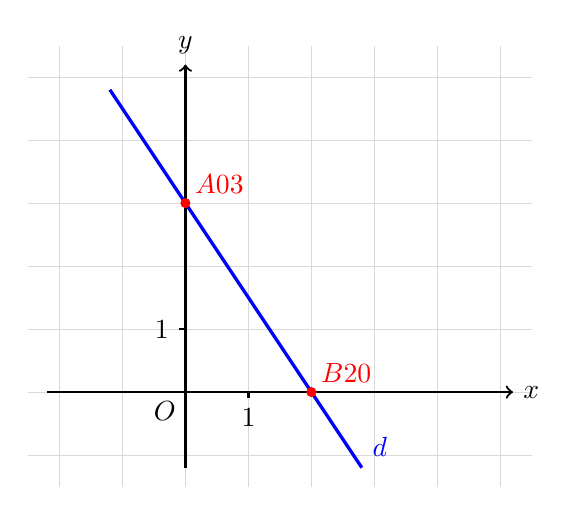
\begin{tikzpicture}[scale=0.8]
			\draw[step=1cm,gray!30,very thin] (-2.5,-1.5) grid (5.5,5.5);
			\draw[thick,->] (-2.2,0) -- (5.2,0) node[right] {$x$};
			\draw[thick,->] (0,-1.2) -- (0,5.2) node[above] {$y$};
			\node[below left] at (0,0) {$O$};
			\draw[thick] (1,0) -- (1,-0.1) node[below] {$1$};
			\draw[thick] (0,1) -- (-0.1,1) node[left] {$1$};
			\draw[line width=1.2pt, blue, domain=-1.2:2.8] plot (\x, {-1.5*\x + 3}) node[above right] {$d$};
			\filldraw[red] (0,3) circle (2pt) node[above right] {$A\coordl{0}{3}$};
			\filldraw[red] (2,0) circle (2pt) node[above right] {$B\coordl{2}{0}$};
		\end{tikzpicture}
	\end{center}
	\begin{remarque}
		Dans cet exemple, nous avons choisi $x = 0$ puis $y = 0$ car la valeur $0$ simplifie grandement les calculs.

		Il est tout à fait possible de choisir n'importe quelle autre valeur pour $x$ (ou pour $y$) pour trouver les points de la droite.
	\end{remarque}
\end{ex}

\begin{prop}[Vecteur directeur et coefficients]
	Soit $(d)$ une droite d'équation cartésienne $ax + by + c = 0$. Le vecteur $\vec{u}\coord{-b}{a}$ est un vecteur directeur de $(d)$.
	\[
		(d) : ax + by + c = 0 \iff \vec{u}\coord{-b}{a} \text{ vecteur directeur de } (d)
	\]
\end{prop}

\begin{demo}
	Soit $A\coordl{x_0}{y_0}$ un point fixé de la droite $d$ et $\vec{u}\coord{\alpha}{\beta}$ un vecteur directeur non nul de $d$.

	Un point $M\coordl{x}{y}$ appartient à la droite $d$ si et seulement si $\vec{AM}\coord{x - x_0}{y - y_0}$ et $\vec{u}\coord{\alpha}{\beta}$ sont colinéaires.

	Or, la colinéarité équivaut à la nullité du déterminant :
	\[
		\def\arraystretch{1.5}
		\begin{array}{rl}
			M \in d & \eqv \determinant{x - x_0                                                        & \alpha \\ y - y_0 & \beta} = 0 \\
			        & \eqv \beta(x - x_0) - \alpha(y - y_0) = 0                                                 \\
			        & \eqv \boxed{\beta} x + \boxed{- \alpha} y + \boxed{(\alpha y_0 - \beta x_0)} = 0
		\end{array}
	\]

	En posant $\boxed{a = \beta}$, $\boxed{b = -\alpha}$ et $\boxed{c = \alpha y_0 - \beta x_0}$, l'équation s'écrit bien sous la forme $ax + by + c = 0$. Puisque $\vec{u} \neq \vec{0}$, le couple $(\alpha\,;\,\beta) \neq (0\,;\,0)$, ce qui garantit $(a\,;\,b) \neq (0\,;\,0)$.

	\ms

	De plus, les coordonnées du vecteur directeur $\vec{u}$ s'expriment sous la forme :
	\[
		\coord{\alpha}{\beta} = \coord{-b}{a}
	\]
\end{demo}

\begin{ex}
	Soit $(d)$ la droite d'équation cartésienne $2x + 3y - 9 = 0$.

	Ici, $a = 2$, $b = 3$ et $c = -9$.

	D'après la propriété, un vecteur directeur de $(d)$ est :
	\[
		\vec{u}\coord{-b}{a} \iff \vec{u}\coord{-3}{2}
	\]

	Pour tracer la droite $(d)$, déterminons deux points à l'aide d'un point initial et du vecteur directeur :
	\begin{itemize}
		\item Pour $x = 0$ :
		      \begin{align*}
			      2\times 0 + 3y - 9 = 0 & \eqv 3y = 9 \\ &\eqv y = 3
		      \end{align*}

		      Donc $A\coordl{0}{3} \in (d)$.
		\item En partant du point $A\coordl{0}{3}$, on applique le vecteur directeur $\vec{u}\coord{-3}{2}$ (déplacement de $-3$ en abscisse et de $+2$ en ordonnée) pour obtenir le point $B\coordl{-3}{5} \in (d)$.
	\end{itemize}

	\begin{center}
		\begin{tikzpicture}[scale=0.85]
			\draw[step=1cm,gray!30,very thin] (-4,-1) grid (6,6);
			\draw[thick,->] (-4.2,0) -- (6.2,0) node[right] {$x$};
			\draw[thick,->] (0,-1.2) -- (0,6.2) node[above] {$y$};
			\node[below left] at (0,0) {$O$};
			\draw[thick] (1,0) -- (1,-0.1) node[below] {$1$};
			\draw[thick] (0,1) -- (-0.1,1) node[left] {$1$};
			\draw[line width=1pt, gray, domain=-4:6] plot (\x, {-2/3*\x + 3}) node[above right] {$(d)$};
			\draw[line width=1.5pt, black, -Stealth] (5,3) -- (2,5) node[midway, above right=-4mm,fill=white] {$\vec{u}\coord{-3}{2}$};
			\draw[line width=1.5pt, black, -Stealth] (5,3) -- (2,5);
			\draw[line width=1.5pt, black, -Stealth] (0,3) -- (-3,5);
			\filldraw[black] (0,3) circle (2.2pt) node[above right] {$A\coordl{0}{3}$};
			\filldraw[black] (-3,5) circle (2.2pt) node[below left, fill=white] {$B\coordl{-3}{5}$};
			\filldraw[black] (-3,5) circle (2.2pt);
			\draw[dashed, black!70, thick] (0,3) -- (-3,3) node[midway, below] {$-3$};
			\draw[dashed, black!70, thick] (-3,3) -- (-3,5) node[midway, left] {$+2$};
		\end{tikzpicture}
	\end{center}
\end{ex}
\begin{remarque}
	L'équation cartésienne d'une droite n'est pas unique.

	Si $ax + by + c = 0$ est une équation cartésienne de $d$, alors pour tout réel $k \neq 0$, $kax + kby + kc = 0$ est aussi une équation cartésienne de $d$.
\end{remarque}

\begin{methode}[Déterminer une équation cartésienne par le déterminant]
	Pour déterminer une équation cartésienne de $d$ connaissant $A\coordl{x_A}{y_A}$ et un vecteur directeur $\vec{u}\coord{u_x}{u_y}$ :

	\begin{enumerate}
		\item Soit $M\coordl{x}{y}$ un point quelconque du plan. Exprimer les coordonnées de $\vec{AM}\coord{x - x_A}{y - y_A}$.
		\item Écrire la condition de colinéarité : $\det\pa{\vec{AM};\vec{u}} = 0$.
		\item Développer et réduire l'expression pour obtenir la forme $ax + by + c = 0$.
	\end{enumerate}
\end{methode}

\begin{exemple}
	Déterminer une équation cartésienne de la droite $d$ passant par $A\coordl{3}{-1}$ et dirigée par le vecteur $\vec{u}\coord{-2}{5}$.

	\begin{correction}
		Soit $M\coordl{x}{y}$ un point du plan. On a $\vec{AM}\coord{x - 3}{y + 1}$.

		\begin{align*}
			M \in d & \eqv \det\pa{\vec{AM};\vec{u}} = 0                          \\
			        & \eqv \determinant{x - 3                                & -2 \\ y + 1 & 5} = 0 \\
			        & \eqv 5(x - 3) - (-2)(y + 1) = 0                             \\
			        & \eqv 5x - 15 + 2y + 2 = 0 \qquad \eqv 5x + 2y - 13 = 0
		\end{align*}

		Une équation cartésienne de la droite $d$ est $5x + 2y - 13 = 0$.

		\begin{center}
			\begin{tikzpicture}[scale=0.65]
				\draw[step=1cm,gray!30,very thin] (-1,-5) grid (6,7);
				\draw[thick,->] (-1,0) -- (6,0) node[above] {$x$};
				\draw[thick,->] (0,-5) -- (0,7) node[right] {$y$};
				\node[below left] at (0,0) {$O$};
				\draw[thick] (1,0) -- (1,-0.1) node[below] {$1$};
				\draw[thick] (0,1) -- (-0.1,1) node[left] {$1$};
				\coordinate (A) at (3,-1);
				\coordinate (M) at (4,-3.5);
				\filldraw[blue!70!black] (M) circle (2.2pt) node[right, fill=white] {$M\coordl{x}{y}$};
				\draw[line width=1.2pt, blue, domain=-0.2:4.6] plot (\x, {-2.5*\x + 6.5}) node[above right] {$d$};
				\filldraw[red] (A) circle (2.2pt) node[right, fill=white] {$A\coordl{3}{-1}$};
				\draw[line width=1.5pt, red, -Stealth] (3,-1) -- (1,4) node[midway, above,sloped, fill=white] {$\vec{u}\coord{-2}{5}$};
				\draw[line width=1.5pt, red, -Stealth] (3,-1) -- (1,4);
				\draw[line width=1.2pt, -Stealth] (A) -- (M) node[midway, below, sloped] {$\vec{AM}$};
				\draw[line width=1.2pt, -Stealth] (A) -- (M);
				\filldraw[red] (A) circle (2.2pt);
				\filldraw[blue!70!black] (M) circle (2.2pt);
				\draw[dashed, red!70, thick] (3,-1) -- (1,-1) node[midway, below] {$-2$};
				\draw[dashed, red!70, thick] (1,-1) -- (1,4) node[midway, left] {$+5$};
			\end{tikzpicture}
		\end{center}
	\end{correction}
\end{exemple}

\subsection{Position relative et critère de parallélisme}

\begin{prop}[Parallélisme via équations cartésiennes]
	Soient deux droites $d$ et $d'$ d'équations cartésiennes respectives $ax + by + c = 0$ et $a'x + b'y + c' = 0$.
	\begin{itemize}
		\item $d\parallel d'$ si et seulement si leurs vecteurs directeurs $\vec{u}\coord{-b}{a}$ et $\vec{u'}\coord{-b'}{a'}$ sont colinéaires, c'est-à-dire :
		      \[
			      \det\pa{\vec{u}~;~\vec{u'}} = 0 \eqv ab' - a'b = 0
		      \]

		\item $d$ et $d'$ sont sécantes si et seulement si $ab' - a'b \neq 0$.
	\end{itemize}
\end{prop}

\begin{exemple}
	Démontrer que les droites $d_1 : 3x - 2y + 5 = 0$ et $d_2 : -6x + 4y + 1 = 0$ sont parallèles.

	\begin{correction}
		Un vecteur directeur de $d_1$ est $\vec{u_1}\coord{2}{3}$. Un vecteur directeur de $d_2$ est $\vec{u_2}\coord{-4}{-6}$.

		Calculons leur déterminant :
		\[
			\det\pa{\vec{u_1}~;~\vec{u_2}} = \determinant{2 & -4 \\ 3 & -6} = 2 \times (-6) - 3 \times (-4) = -12 + 12 = 0
		\]

		Les vecteurs $\vec{u_1}$ et $\vec{u_2}$ sont colinéaires, donc les droites $d_1$ et $d_2$ sont parallèles.

		\begin{center}
			\begin{tikzpicture}[scale=0.85]
				\draw[step=1cm,gray!30,very thin] (-4.5,-2.5) grid (4.5,5.5);
				\draw[thick,->] (-4.2,0) -- (4.3,0) node[right] {$x$};
				\draw[thick,->] (0,-2.2) -- (0,5.3) node[above] {$y$};
				\node[below left] at (0,0) {$O$};
				\draw[thick] (1,0) -- (1,-0.1) node[below] {$1$};
				\draw[thick] (0,1) -- (-0.1,1) node[left] {$1$};
				\draw[line width=1.2pt, blue, domain=-3.2:1.7] plot (\x, {1.5*\x + 2.5}) node[above right] {$d_1$};
				\draw[line width=1.2pt, orange, domain=-1.3:3.6] plot (\x, {1.5*\x - 0.25}) node[above right] {$d_2$};
				\draw[line width=1.5pt, red, -Stealth] (-1,1) -- (1,4) node[midway, above left,fill=white] {$\vec{u}_1\coord{2}{3}$};
				\filldraw[blue] (-1,1) circle (3pt);
				\draw[line width=1.5pt, codegreen, -Stealth] (3,4.25) -- (-1,-1.75) node[midway, below right, fill=white, yshift=4mm] {$\vec{u}_2\coord{-4}{-6}$};
				\draw[line width=1.5pt, codegreen, -Stealth] (3,4.25) -- (-1,-1.75);
				\filldraw[orange] (3,4.25) circle (3pt);
			\end{tikzpicture}
		\end{center}
	\end{correction}
\end{exemple}

\begin{remarque}
	Une droite sécante à l'axe des ordonnées d'équation $y = mx + p$ admet pour vecteur directeur $\vec{u}\coord{1}{m}$.
\end{remarque}

\begin{methode}[Passer de l'équation cartésienne à l'équation réduite]
	Soit la droite $d$ d'équation cartésienne $ax + by + c = 0$.
	\begin{itemize}
		\item Si $b = 0$, alors $a \neq 0$ et l'équation s'écrit $ax + c = 0$, soit $x = \dfrac{-c}{a}$.

		      C'est une droite parallèle à l'axe des ordonnées.
		\item Si $b \neq 0$, on isole $y$ dans l'équation :
		      \[
			      by = -ax - c \eqv y = -\frac{a}{b}x - \frac{c}{b}
		      \]

		      On identifie alors la pente $m = \dfrac{-a}{b}$ et l'ordonnée à l'origine $p = \dfrac{-c}{b}$.
	\end{itemize}
\end{methode}

\section{Exercices types}

\begin{exercice}
	Soient $A\coordl{-2}{1}$, $B\coordl{1}{3}$ et $C\coordl{4}{5}$ trois points du plan.
	\begin{enumerate}
		\item Déterminer une équation cartésienne de la droite $(AB)$.
		\item Les points $A$, $B$ et $C$ sont-ils alignés ?
	\end{enumerate}
\end{exercice}

\begin{correction}
	\nline
	\begin{enumerate}
		\item Le vecteur $\vec{AB}$ a pour coordonnées $\coord{1 - (-2)}{3 - 1} = \coord{3}{2}$. Soit $M\coordl{x}{y}$ un point du plan.
		      \begin{align*}
			      M \in (AB) & \eqv \determinant{\vec{AM}   & \vec{AB}} = 0 \\
			                 & \eqv \determinant{x + 2      & 3             \\ y - 1 & 2} = 0 \\
			                 & \eqv 2(x + 2) - 3(y - 1) = 0                 \\
			                 & \eqv 2x + 4 - 3y + 3 = 0                     \\
			                 & \eqv 2x - 3y + 7 = 0
		      \end{align*}

		      Une équation cartésienne de $(AB)$ est $2x - 3y + 7 = 0$.

		\item Testons si les coordonnées du point $C\coordl{4}{5}$ vérifient cette équation :
		      \[
			      2x_C - 3y_C + 7 = 2(4) - 3(5) + 7 = 8 - 15 + 7 = 0
		      \]

		      Les coordonnées de $C$ vérifient l'équation de la droite $(AB)$, donc $C \in (AB)$.

		      Par conséquent, les points $A$, $B$ et $C$ sont alignés.
	\end{enumerate}
\end{correction}

\begin{exercice}
	On considère les droites $d_1 : 4x - 6y + 3 = 0$ et $d_2 : y = \frac{2}{3}x - 5$.
	\begin{enumerate}
		\item Déterminer l'équation réduite de $d_1$.
		\item Étudier la position relative de $d_1$ et $d_2$.
	\end{enumerate}
\end{exercice}

\begin{correction}
	\nline
	\begin{enumerate}
		\item Pour la droite $d_1$, isolons $y$ :
		      \[
			      \def\arraystretch{2}
			      \begin{array}{rcl}
				      4x - 6y + 3 = 0 & \eqv & 6y = 4x + 3                      \\
				                      & \eqv & y = \dfrac{4}{6}x + \dfrac{3}{6} \\
				                      & \eqv & y = \dfrac{2}{3}x + \dfrac{1}{2}
			      \end{array}
		      \]

		      L'équation réduite de $d_1$ est $y = \dfrac{2}{3}x + \dfrac{1}{2}$.

		\item Le coefficient directeur de $d_1$ est $m_1 = \dfrac{2}{3}$ et celui de $d_2$ est $m_2 = \dfrac{2}{3}$.

		      Puisque $m_1 = m_2$, les droites $d_1$ et $d_2$ sont parallèles.

		      De plus, leurs ordonnées à l'origine sont différentes ($\dfrac{1}{2} \neq -5$), donc $d_1$ et $d_2$ sont strictement parallèles.
	\end{enumerate}
\end{correction}

% ----------------------------------------------------------------------------------------------------
\newpage
\section{Exercices}
 {\small
  \begin{multicols}{2}
	  \begin{exo}{}
	Dans chaque cas, déterminer deux vecteurs directeurs de la droite $d$ dont une équation est donnée ci-dessous.

	\vspace*{-2mm}\begin{multicols}{2}
		\begin{enumerate}
			\item $3x - 4y + 1 = 0$
			\item $y = 2$
			\item $x = 3$
			\item $-2x + 7y + 5 = 0$
		\end{enumerate}
	\end{multicols}
\end{exo}

	  \begin{exo}{}
	Dans chaque cas, déterminer le coefficient directeur de la droite $d$ dont une équation est donnée ci-dessous.

	\vspace*{-2mm}\begin{multicols}{2}
		\begin{enumerate}
			\item $-4x + 2y + 1 = 0$
			\item $x - 3y = 0$
			\item $5x - 5y - 5 = 0$
			\item $2x - 5y + 15 = 0$
		\end{enumerate}
	\end{multicols}
\end{exo}

	  \begin{exo}{}
	Dans chaque cas, déterminer le coefficient directeur de la droite $(AB)$ :

	\begin{enumerate}
		\item $A\coordl{1}{2}$ et $B\coordl{2}{5}$
		\item $A\coordl{-5}{1}$ et $B\coordl{-1}{0}$
		\item $A\coordl{-0,5}{3}$ et $B\coordl{0,5}{-2}$
		\item $A\coordl{\dfrac{-2}{3}}{\dfrac{1}{4}}$ et $B\coordl{\dfrac{1}{3}}{1,25}$
		\item $A\coordl{0}{0}$ et $B\coordl{4}{4}$
	\end{enumerate}
\end{exo}

	  \begin{exo}{}
	\begin{center}
		\begin{tikzpicture}[scale=0.7, >=Stealth]
			\def\xmin{-5.5}\def\xmax{4.5}\def\ymin{-0.8}\def\ymax{8.5}
			\clip (\xmin, \ymin) rectangle (\xmax, \ymax);
			\draw[xstep=1, gray!40, ystep=1] (\xmin, \ymin) grid (\xmax, \ymax);
			\draw[->, very thick] (\xmin, 0) -- (\xmax, 0) node[above left] {$x$};
			\draw[->, very thick] (0, \ymin) -- (0, \ymax) node[below right] {$y$};
			\foreach \x in {-5,-4,-3,-2,-1,1,2,3,4}
			\draw (\x,0.1) -- (\x,-0.1);
			\foreach \y in {1,2,3,4,5,6,7,8,9,10}
			\draw (0.1,\y) -- (-0.1,\y);
			\node[below left, scale=0.8] at (0,0) {$O$};
			\draw[->, very thick, black] (0,0) -- (1,0) node[midway, below, scale=0.8] {$\vec{i}$};
			\draw[->, very thick, black] (0,0) -- (0,1) node[midway, left, scale=0.8] {$\vec{j}$};
			\node[red,fill=white] at (4, 6.9) {$d_1$};
			\node[vert, fill=white] at (-1.8, 1) {$d_2$};
			\node[bleu, right, fill=white] at (1.9, 2.5) {$d_3$};
			\node[purple,fill=white] at (-5, 5.7) {$d_4$};
			\draw[domain=\xmin:\xmax, smooth, very thick, red] plot (\x, {1/3*\x + 6});
			\draw[domain=-4.5:0, smooth, very thick, vert] plot (\x, {-3*\x - 3});
			\draw[domain=\xmin:\xmax, smooth, very thick, purple] plot (\x, {-0.75*\x + 1.5 });
			\draw[very thick, bleu] (2, \ymin) -- (2, \ymax);
			% \foreach \pt in {(0,6), (-3,5), (-1,0), (-2,3), (2,0)} { \filldraw[black] \pt circle (3pt); }
		\end{tikzpicture}
	\end{center}

	\begin{enumerate}
		\item Donner deux vecteurs directeurs de chacune des droites tracées.
	\end{enumerate}
\end{exo}

	  \begin{exo}{}
	Dans chacun des cas suivants, indiquer si le vecteur $\vec{u}$ est un vecteur directeur de la droite $(AB)$.
	\begin{enumerate}
		\item $A\coordl{1}{0}$ et $B\coordl{0}{1}$\ ;\ $\vec{u}\coord{1}{1}$
		\item $A\coordl{2}{3}$ et $B\coordl{-3}{4}$\ ;\ $\vec{u}\coord{5}{-1}$
		\item $A\coordl{-1}{4}$ et $B\coordl{-2}{6}$\ ;\ $\vec{u}\coord{2}{1}$
		\item $A\coordl{4}{-2}$ et $B\coordl{1}{1}$\ ;\ $\vec{u}\coord{1}{-1}$
	\end{enumerate}
\end{exo}

	  \vfill~\columnbreak
	  \begin{exo}{}
	On se place dans un repère orthonormé $\vOIJ$.

	\begin{center}
		\begin{tikzpicture}[scale=0.55, >=Stealth]
			\def\xmin{-3.5}\def\xmax{7.5}\def\ymin{-4.5}\def\ymax{6.5}
			\clip (\xmin, \ymin) rectangle (\xmax, \ymax);
			\draw[xstep=1, gray!40, ystep=1] (\xmin, \ymin) grid (\xmax, \ymax);
			\draw[->, very thick] (\xmin, 0) -- (\xmax, 0) node[above left] {$x$};
			\draw[->, very thick] (0, \ymin) -- (0, \ymax) node[below right] {$y$};
			\foreach \x in {-3,-2,-1,1,2,3,4,5,6,7}
			\draw (\x,0.1) -- (\x,-0.1);
			\foreach \y in {-5,-4,-3,-2,-1,1,2,3,4,5,6}
			\draw (0.1,\y) -- (-0.1,\y);
			\node[below left, scale=0.8] at (0,0) {$O$};
			\draw[->, very thick, black] (0,0) -- (1,0) node[midway, below, scale=0.8] {$\vec{i}$};
			\draw[->, very thick, black] (0,0) -- (0,1) node[midway, left, scale=0.8] {$\vec{j}$};
			\node[violet, fill=white, above] at (5, 5.4) {$d_1$};
			\node[vert, fill=white, left] at (-0.5, 5) {$d_2$};
			\node[orange, fill=white, below right] at (6, 5.5) {$d_3$};
			\node[teal, fill=white, left] at (-2, 2) {$d_4$};
			\node[purple, fill=white, below] at (-1.5, -3) {$d_5$};
			\node[bleu, fill=white, above left] at (4, 5.2) {$d_6$};
			\draw[domain=\xmin:\xmax, smooth, very thick, violet] plot (\x, {\x});
			\draw[domain=-1.5:5, smooth, very thick, vert] plot (\x, {-2*\x + 4});
			\draw[domain=\xmin:\xmax, smooth, very thick, orange] plot (\x, {0.75*\x + 1});
			\draw[domain=-3.5:2, smooth, very thick, teal] plot (\x, {-2*\x - 2});
			\draw[very thick, purple] (\xmin, -3) -- (\xmax, -3);
			\draw[very thick, bleu] (4, \ymin) -- (4, \ymax);
		\end{tikzpicture}
	\end{center}

	\begin{enumerate}
		\item Déterminer les coordonnées d'un vecteur directeur pour chacune des droites représentées ci-dessus.
	\end{enumerate}
\end{exo}

	  \begin{exo}{}
	On considère l'équation réduite d'une droite $d$ définie par $y = ax + b$ représentée dans le repère ci-dessous :

	\begin{center}
		\begin{tikzpicture}[scale=0.40, >=Stealth]
			\def\xmin{-7.5}\def\xmax{7.5}\def\ymin{-4.5}\def\ymax{6.5}
			\clip (\xmin, \ymin) rectangle (\xmax, \ymax);
			\draw[xstep=1, gray!40, ystep=1] (\xmin, \ymin) grid (\xmax, \ymax);
			\draw[->, very thick] (\xmin, 0) -- (\xmax, 0) node[above left] {$x$};
			\draw[->, very thick] (0, \ymin) -- (0, \ymax) node[below right] {$y$};
			\draw (-5,0.2) -- (-5,-0.2) node[below,fill=white, scale=0.8] {$-5$};
			\draw (1,0.2) -- (1,-0.2) node[below,fill=white, scale=0.8] {$1$};
			\draw (5,0.2) -- (5,-0.2) node[below,fill=white, scale=0.8] {$5$};
			\draw (0.2,1) -- (-0.2,1) node[left,fill=white, scale=0.8] {$1$};
			\draw (0.2,5) -- (-0.2,5) node[left,fill=white, scale=0.8] {$5$};
			\node[below left, scale=0.8] at (0,0) {$0$};
			\fill[teal!20, opacity=0.6] (3,3) -- (6,3) -- (6,5) -- cycle;
			\draw[thick, teal] (3,3) -- (6,3) node[midway, below, scale=0.9, font=\bfseries] {3};
			\draw[thick, teal] (6,3) -- (6,5) node[midway, right, scale=0.9, font=\bfseries] {2};
			\fill[teal!20, opacity=0.6] (-6,-3) -- (-6,1) -- (0,1) -- cycle;
			\draw[thick, teal] (-6,-3) -- (-6,1) node[midway, left, scale=0.9, font=\bfseries] {4};
			\draw[thick, teal] (-6,1) -- (0,1) node[midway, above, scale=0.9, font=\bfseries] {6};
			\draw[domain=\xmin:\xmax, smooth, very thick, blue!70!black] plot (\x, {2/3*\x + 1});
			\filldraw[black] (0,1) circle (2pt);
		\end{tikzpicture}
	\end{center}

	\begin{enumerate}
		\item Avec les indications de la figure, proposer deux calculs pour la valeur du coefficient directeur.
		\item En quel point la droite coupe-t-elle l'axe des ordonnées ?
	\end{enumerate}
\end{exo}

	  \begin{exo}{}
	Les points orange appartiennent à une droite d'équation $y = mx + p$.

	\begin{center}
		\begin{tikzpicture}[scale=0.40, >=Stealth]
			\def\xmin{-6.5}\def\xmax{7.5}\def\ymin{-3.5}\def\ymax{6.5}
			\clip (\xmin, \ymin) rectangle (\xmax, \ymax);
			\draw[xstep=1, gray!40, ystep=1] (\xmin, \ymin) grid (\xmax, \ymax);
			\draw[very thick] (\xmin, 0) -- (\xmax, 0) node[above left] {$x$};
			\draw[very thick] (0, \ymin) -- (0, \ymax) node[below right] {$y$};
			\foreach \x in {-6,-5,-4,-3,-2,-1,1,2,3,4,5,6,7,8,9} \draw (\x,0.2) -- (\x,-0.2);
			\foreach \y in {-4,-3,-2,-1,1,2,3,4,5,6} \draw (0.2,\y) -- (-0.2,\y);
			\draw[->, thick, black] (0,0) -- (1,0) node[midway, below, scale=0.8] {$\vec{i}$};
			\draw[->, thick, black] (0,0) -- (0,1) node[midway, left, scale=0.8] {$\vec{j}$};
			\draw[domain=\xmin:\xmax, smooth, very thick, green!60!black] plot (\x, {0.75*\x + 1.5});
			\foreach \coord in {(-6,-3), (-2,0), (2,3), (6,6)} { \filldraw[orange] \coord circle (5pt); }
		\end{tikzpicture}
	\end{center}

	\begin{enumerate}
		\item Avec les indications de la figure, proposer des calculs pour déterminer $m$.
		\item Quelle est l'ordonnée du point d'abscisse $5$ ?
	\end{enumerate}
\end{exo}

	  \begin{exo}{}
	Les points orange appartiennent à la droite d'équation $y = mx + p$.

	\begin{center}
		\begin{tikzpicture}[>=Stealth,x=2.5mm,y=4mm]
			\def\xmin{-17.5}\def\xmax{14.5}\def\ymin{-3.5}\def\ymax{9}
			\clip (\xmin, \ymin) rectangle (\xmax, \ymax);
			\draw[xstep=5, gray!40, ystep=2] (\xmin, \ymin) grid (\xmax, \ymax);
			\draw[->, very thick] (\xmin, 0) -- (\xmax, 0) node[above left] {$x$};
			\draw[->, very thick] (0, \ymin) -- (0, \ymax) node[below right] {$y$};
			\draw (-15,0.2) -- (-15,-0.2) node[below,fill=white, scale=0.9] {$-15$};
			\draw (5,0.2) -- (5,-0.2) node[below,fill=white, scale=0.9] {$5$};
			\draw (0.2,2) -- (-0.2,2) node[left,fill=white, scale=0.9] {$2$};
			\draw (0.2,8) -- (-0.2,8) node[left,fill=white, scale=0.9] {$8$};
			\draw[domain=\xmin:\xmax, smooth, very thick, gray] plot (\x, {-0.4*\x + 2});
			\foreach \coord in {(-10,6), (-5,4), (10,-2)} { \filldraw[orange] \coord circle (2pt); }
		\end{tikzpicture}
	\end{center}

	\begin{enumerate}
		\item Avec les indications de la figure, proposer des calculs pour déterminer $m$.
		\item Quelle est l'ordonnée du point d'abscisse $25$ ?
	\end{enumerate}
\end{exo}

	  \begin{exo}{}
	Dans chaque cas, déterminer l'équation réduite de la droite dont on donne une équation cartésienne.
	\vspace*{-2mm}\begin{multicols}{2}
		\begin{enumerate}
			\item $-2x + y + 1 = 0$
			\item $-1,5x + 3y - 4,5 = 0$
			\item $\dfrac{-7}{3}y - 3 = 0$
		\end{enumerate}
	\end{multicols}
\end{exo}

	  \begin{exo}{}
	Déterminer l'équation réduite de la droite passant par $A$ et de coefficient directeur $m$.
	\begin{enumerate}
		\item $A\coordl{5}{2}$ et $m = -3$
		\item $A\coordl{-4}{-1}$ et $m = \dfrac{1}{2}$
		\item $A\coordl{-\dfrac{1}{7}}{\dfrac{3}{7}}$ et $m = 2$
	\end{enumerate}
\end{exo}

	  \begin{exo}{}
	Dans chaque cas, déterminer une équation de $(AB)$.
	\begin{enumerate}
		\item $A\coordl{-6}{-1}$ et $B\coordl{3}{3}$
		\item $A\coordl{5}{0}$ et $B\coordl{5}{2}$
		\item $A\coordl{4}{-\dfrac{7}{9}}$ et $B\coordl{0}{\dfrac{2}{9}}$
	\end{enumerate}
\end{exo}

	  \begin{exo}{}
	Déterminer une équation de la droite passant par $A$ et de vecteur directeur $\vec{u}$.
	\begin{enumerate}
		\item $A\coordl{0}{4}$ et $\vec{u}\coord{4}{-1}$
		\item $A\coordl{5}{2}$ et $\vec{u}\coord{-2}{1}$
		\item $A\coordl{-3}{0}$ et $\vec{u}\coord{0}{5}$
	\end{enumerate}
\end{exo}

	  \vfill~\columnbreak
	  \begin{exo}{}
	On se place dans un repère orthonormé $\vOIJ$.

	Déterminer l'équation réduite de chacune des droites ci-dessous, sous la forme $y = mx + p$ ou $x = c$.

	\begin{center}
		\begin{tikzpicture}[scale=0.8, >=Stealth]
			\def\xmin{-4.5}\def\xmax{3.5}\def\ymin{-3.5}\def\ymax{3.5}
			\clip (\xmin, \ymin) rectangle (\xmax, \ymax);
			\draw[xstep=1, gray!40, ystep=1] (\xmin, \ymin) grid (\xmax, \ymax);
			\draw[very thick] (\xmin, 0) -- (\xmax, 0);
			\draw[very thick] (0, \ymin) -- (0, \ymax);
			\foreach \x in {-4,-3,-2,-1,1,2,3} \draw (\x,0.1) -- (\x,-0.1);
			\foreach \y in {-3,-2,-1,1,2,3} \draw (0.1,\y) -- (-0.1,\y);
			\node[below left, scale=0.8] at (0,0) {$O$};
			\draw[->, thick, black] (0,0) -- (1,0) node[midway, below, scale=0.8] {$\vec{i}$};
			\draw[->, thick, black] (0,0) -- (0,1) node[midway, left, scale=0.8] {$\vec{j}$};
			\node[bleu, fill=white, below right] at (2.5, 2.4) {$d_1$};
			\node[vert, fill=white, above left] at (2, 2.5) {$d_2$};
			\node[orange, fill=white, above left] at (-1, 2.5) {$d_3$};
			\node[red, fill=white, above left] at (3.5, -3) {$d_4$};
			\draw[very thick, red] (\xmin, -3) -- (\xmax, -3);
			\draw[domain=\xmin:\xmax, smooth, very thick, bleu] plot (\x, {0.5*\x + 1});
			\draw[very thick, vert] (2, \ymin) -- (2, \ymax);
			\draw[very thick, orange] (-1, \ymin) -- (-1, \ymax);
		\end{tikzpicture}
	\end{center}
\end{exo}

	  \begin{exo}{}
	On se place dans un repère orthonormé $\vOIJ$.

	Par lecture graphique, déterminer une équation cartésienne de chacune des droites représentées dans le repère ci-dessous.

	\begin{center}
		\begin{tikzpicture}[scale=0.65, >=Stealth]
			\def\xmin{-5.5}\def\xmax{7.5}\def\ymin{-3.5}\def\ymax{4.5}
			\clip (\xmin, \ymin) rectangle (\xmax, \ymax);
			\draw[xstep=1, gray!40, ystep=1] (\xmin, \ymin) grid (\xmax, \ymax);
			\draw[very thick] (\xmin, 0) -- (\xmax, 0);
			\draw[very thick] (0, \ymin) -- (0, \ymax);
			\foreach \x in {-5,-4,-3,-2,-1,1,2,3,4,5,6,7} \draw (\x,0.1) -- (\x,-0.1);
			\foreach \y in {-3,-2,-1,1,2,3,4} \draw (0.1,\y) -- (-0.1,\y);
			\node[below left, scale=0.8] at (0,0) {$O$};
			\draw[->, thick, black] (0,0) -- (1,0) node[midway, below, scale=0.8] {$\vec{i}$};
			\draw[->, thick, black] (0,0) -- (0,1) node[midway, left, scale=0.8] {$\vec{j}$};
			\node[violet, fill=white, above] at (-4.5, -1) {$d_1$};
			\node[vert, fill=white, left] at (-2, 3.5) {$d_2$};
			\node[orange, fill=white, above right] at (-4.2, 2) {$d_3$};
			\node[teal, fill=white, below right] at (-4.5, -2.1) {$d_4$};
			\node[magenta, fill=white, right] at (1.3, -2) {$d_5$};
			\draw[domain=\xmin:\xmax, smooth, very thick, violet] plot (\x, {-1});
			\draw[very thick, vert] (-2, \ymin) -- (-2, \ymax);
			\draw[domain=\xmin:\xmax, smooth, very thick, orange] plot (\x, {-\x - 2});
			\draw[domain=\xmin:\xmax, smooth, very thick, teal] plot (\x, {0.5*\x});
			\draw[domain=\xmin:\xmax, smooth, very thick, magenta] plot (\x, {\x - 3});
		\end{tikzpicture}
	\end{center}
\end{exo}

	  \begin{exo}{}
	Dans chacun des cas suivants, déterminer une équation cartésienne de la droite $d$ parallèle à la droite $(AB)$ et passant par le point $C$ :
	\begin{enumerate}
		\item $A\coordl{1}{0}$, $B\coordl{0}{1}$ et $C\coordl{3}{-2}$
		\item $A\coordl{1}{-3}$, $B\coordl{2}{1}$ et $C\coordl{1}{1}$
		\item $A\coordl{-2}{-2}$, $B\coordl{1}{-5}$ et $C\coordl{-6}{2}$
		\item $A\coordl{-5}{1}$, $B\coordl{-1}{-1}$ et $C\coordl{-2}{-2}$
	\end{enumerate}
\end{exo}

	  \begin{exo}{}
	Tracer dans un repère les droites suivantes :
	\begin{enumerate}
		\item $d_1 : y = 2x + 1$
		\item $d_2 : y = 0,5x$
		\item $d_3 : y = 3x - 2$
		\item $d_4 : y = \dfrac{1}{4}x - 1$
	\end{enumerate}
\end{exo}

	  \vfill~\columnbreak
	  \begin{exo}{}
	Dans un repère orthonormé, tracer les droites suivantes :
	\begin{enumerate}
		\item $d_1$ d'équation cartésienne $-x + 2y + 4 = 0$.
		\item $d_2$ passant par $A\coordl{-4}{2}$ et de vecteur directeur $\vec{u}\coord{4}{-3}$.
		\item $d_3$ d'équation réduite $y = -x + 4,5$.
		\item $d_4$ passant par $B\coordl{-2}{4}$ et de coefficient directeur $-1,5$.
	\end{enumerate}
\end{exo}

	  \begin{exo}{}
	Représenter dans un repère la droite passant par le point $A$ et de vecteur directeur $\vec{u}$.
	\begin{enumerate}
		\item Droite $d_1$ : $A\coordl{1}{1}$ et $\vec{u}\coord{-1}{3}$
		\item Droite $d_2$ : $A\coordl{-2}{1}$ et $\vec{u}\coord{5}{1}$
		\item Droite $d_3$ : $A\coordl{0}{3}$ et $\vec{u}\coord{3}{0}$
		\item Droite $d_4$ : $A\coordl{-4}{0}$ et $\vec{u}\coord{0}{5}$
	\end{enumerate}
\end{exo}

	  \begin{exo}{}
	Représenter dans le repère chacune des droites suivantes dont on donne une équation cartésienne :
	\vspace*{-2mm}
	\begin{multicols}{2}
		\begin{enumerate}
			\item $d_1 : x + y + 1 = 0$
			\item $d_2 : 2x - y - 2 = 0$
			\item $d_3 : -x + 2y + 3 = 0$
			\item $d_4 : 3x - 2y + 3 = 0$
			\item $d_5 : 2x + 3y - 4 = 0$
		\end{enumerate}
	\end{multicols}
\end{exo}

	  \begin{exo}{}
	Démontrer que les points $A$, $B$ et $C$ sont alignés :
	\cmath{A\coordl{100}{1500}\text{, }B\coordl{180}{1900}\text{ et }C\coordl{198}{1990}}
\end{exo}

	  \begin{exo}{}
	Dans chacun des cas suivants, déterminer en justifiant si les points $A$, $B$ et $C$ sont alignés :
	\begin{enumerate}
		\item $A\coordl{-4}{-4}$, $B\coordl{0}{0}$ et $C\coordl{4}{4}$
		\item $A\coordl{-2}{3}$, $B\coordl{1}{0}$ et $C\coordl{4}{1}$
		\item $A\coordl{5}{2}$, $B\coordl{0}{2}$ et $C\coordl{1}{2}$
		\item $A\coordl{4}{-2}$, $B\coordl{4}{3}$ et $C\coordl{0}{3}$
	\end{enumerate}
\end{exo}

	  \vfill~\columnbreak
	  \begin{exo}{}
	$ABCD$ est un carré dont le côté mesure $4$ cm. $DFC$ et $BCH$ sont des triangles équilatéraux.

	\begin{center}
		\begin{tikzpicture}[scale=0.5, >=Stealth]
			\coordinate (A) at (0,0);
			\coordinate (B) at (4,0);
			\coordinate (C) at (4,4);
			\coordinate (D) at (0,4);
			\coordinate (F) at (2, {4 + 2*sqrt(3)});
			\coordinate (H) at ({4 - 2*sqrt(3)}, 2);
			\draw[thick] (A) -- (B) -- (C) -- (D) -- cycle;
			\draw[thick] (D) -- (F) -- (C);
			\draw[thick] (B) -- (H) -- (C);
			\node[below left] at (A) {$A$};
			\node[below right] at (B) {$B$};
			\node[right] at (C) {$C$};
			\node[left] at (D) {$D$};
			\node[above] at (F) {$F$};
			\node[above] at (H) {$H$};
			\foreach \pt in {A, B, C, D, F, H} { \filldraw (\pt) circle (3pt); }
		\end{tikzpicture}
	\end{center}

	\begin{enumerate}
		\item Calculer la hauteur de chaque triangle équilatéral.
		\item Démontrer que les points $A$, $H$ et $F$ sont alignés.
	\end{enumerate}

	\textit{Aide : On pourra se placer dans un repère convenablement choisi.}
\end{exo}

	  \begin{exo}{}
	Dans chaque cas, déterminer si les droites $d$ et $d'$ sont strictement parallèles, sécantes ou confondues.
	\begin{enumerate}
		\item $d : 3x - 2y + 7 = 0$ et $d' : 3x + 2y - 7 = 0$
		\item $d : \dfrac{7}{3}x - y + 2 = 0$ et $d' : 7x - 3y + 9 = 0$
		\item $d : x + 7 = 0$ et $d' : -5x - 35 = 0$
	\end{enumerate}
\end{exo}

	  \begin{exo}{}
	Dans chaque cas, déterminer, sans la tracer, si la droite $(AB)$ est parallèle à l'un des axes ou non. Si oui, lequel ?
	\begin{enumerate}
		\item $A\coordl{3}{3}$ et $B\coordl{3}{1}$
		\item $A\coordl{1}{-1}$ et $B\coordl{2}{-1}$
		\item $A\coordl{0,5}{0,25}$ et $B\coordl{0,25}{0,5}$
		\item $A\coordl{0,25}{2}$ et $B\coordl{\dfrac{1}{4}}{\dfrac{4}{8}}$
	\end{enumerate}
\end{exo}

	  \begin{exo}{}
	Dans chaque cas, déterminer une équation cartésienne de la droite $d'$ parallèle à la droite $d$ et passant par le point $A$ :
	\begin{enumerate}
		\item $d : 2x + y + 3 = 0$ et $A\coordl{-1}{5}$
		\item $d : x + y = 0$ et $A\coordl{7}{1}$
		\item $d : x = 4$ et $A\coordl{3}{0}$
		\item $d : y = \dfrac{1}{2}x - \dfrac{1}{4}$ et $A\coordl{-3}{2}$
	\end{enumerate}
\end{exo}

	  \vfill~
  \end{multicols}
 }

